\noindent En la \cref{ratios} se observa la razón de tiempos entre los algoritmos de Fuerza Bruta y Programación Dinámica en los diferentes casos de prueba.

\begin{itemize}
    \item \textbf{Valores superiores a 1:} Indican que el algoritmo de Fuerza Bruta es más lento que el de Programación Dinámica para ese caso.
    
    \item \textbf{Valores cercanos a 1:} Indican que ambos algoritmos tienen tiempos similares para ese caso.
    
    \item \textbf{Valores inferiores a 1:} Indican que el algoritmo de Fuerza Bruta es más rápido que el de Programación Dinámica.
\end{itemize}

\begin{figure}[H]
    \centering
    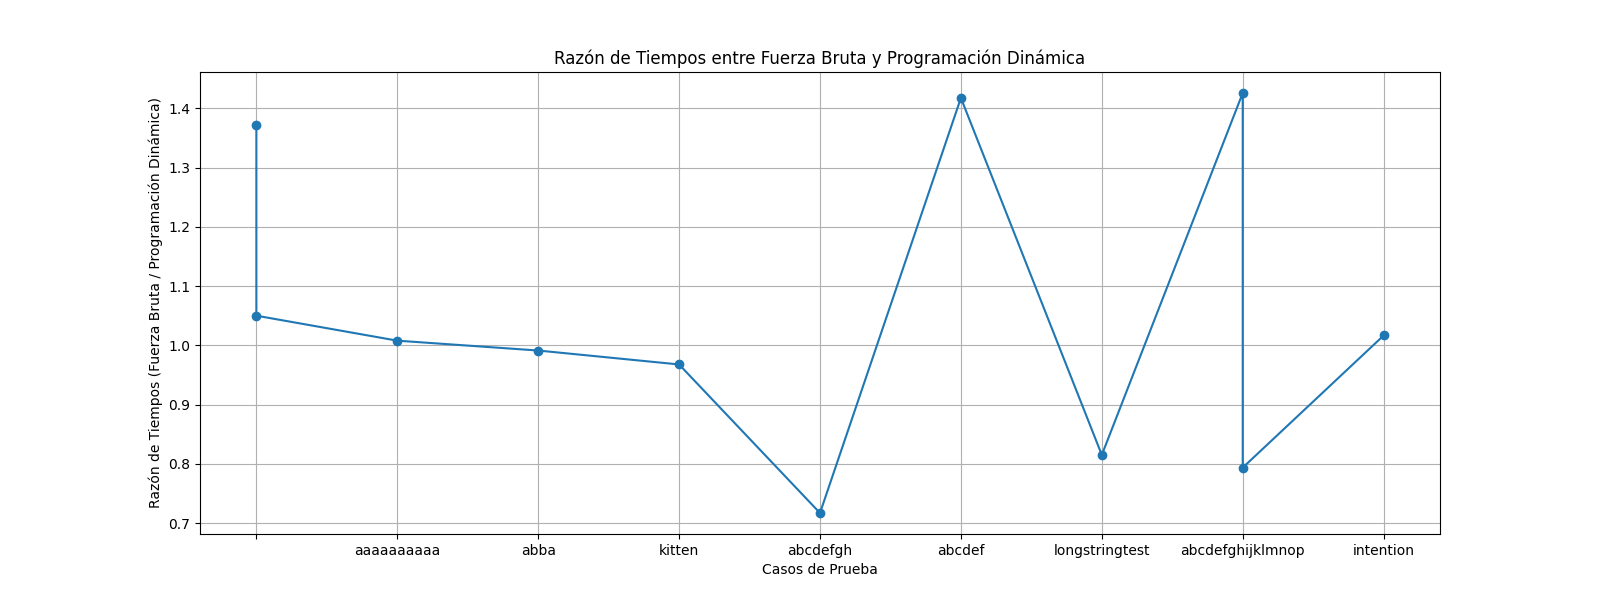
\includegraphics[width=\textwidth]{images/speedup_ratio.png}
    \caption{Razón de los tiempos entre BF y DP.}
    \label{ratios}
\end{figure}
